\documentclass{ctexart}

\usepackage{bm}
\usepackage{amsmath}
\usepackage{lmodern}
\usepackage{graphicx}

\title{针对密集物体检测的焦点损失}
\date{2018 \\ February}
\author{Tsung-Yi Lin, Priya Goyal, Ross Girshick, Kaiming He, Piotr Dollar
\and Facebook AI Research (FAIR)}
\begin{document}
\maketitle
\begin{figure}[h] \label{fig:focal_loss}
    \centering
    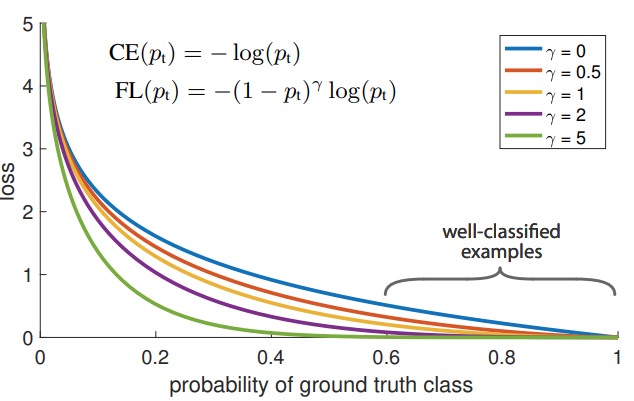
\includegraphics[width=.8\textwidth]{images/focal_loss.png}
    \caption{我们提出了一个名为焦点误差的损失,它在标准的交叉熵损失上加入了一个$(1-p_t)^\gamma$因子。设置$\gamma > 0$将会减少对于分类良好($p_t > .5$)例子的相对损失,从而更加专注于难的、错误分类的例子。正如我们的实验将要阐明的,我们提出的焦点误差使得在存在大量简单背景例子的情况下可以训练得到高精度密集物体检测器。}
\end{figure}
\begin{abstract}
    目前精度最高的检测器是由R-CNN普及、基于双阶段方法的,其中一个分类器被应用在一系列稀疏的候选物体位置上。与之相较的是,在物体可能位置的常规密集采样的单阶段检测器有更快和更简便的潜能,但是与双阶段的检测器精度相差较远。在这篇文章中,我们调研了这种情况的原因。我们发现在训练密集检测器过程中遇到的前景背景类别的极度不平衡是重要原因。我们通过重塑标准的交叉熵损失,降低分类良好的实例的损失的权重来解决这个类别不平衡问题。我们的焦点损失专注于在一系列稀疏的难例上训练,并防止了大量简单的负例在训练过程中压倒检测器。为了评估我们的损失的有效性,我们设计并训练了一个我们起名为RetinaNet的密集检测器。结果显示,当我们使用焦点损失训练时,RetinaNet可以匹配单阶段检测器的速度同时超过所有现有两阶段检测器的精度。
\end{abstract}
\section{introduction}
现有的sota物体检测器是基于两阶段的候选区域驱动机制的。正如R-CNN框架中所普及的,第一个阶段生成稀疏的候选物体位置,第二阶段使用卷积神经网络将每一个候选位置分类为某一种前景或者背景。通过一系列的改进,双阶段框架始终在COCO基准数据集上达到高准确度。\newline
尽管双阶段检测器获得了成功,但是一个自然的问题是:简单的单阶段检测器可以达到相似的准确率吗?单阶段检测器被应用在物体位置、尺寸和长宽比的普通的密集采样上。近期单阶段检测器的工作,例如YOLO和SSD,展示了光明的结果,得到了精度为sota双阶段检测器10\%到40\%的更快速的检测器。\newline
这篇文章更进一步推动了信封:开创性地,我们提出了一个可以匹配更加复杂的双阶段检测器例如特征金字塔网络(FPN)或者Faster R-CNN的变种Mask R-CNN,的最好COCO平均精度的单阶段检测器。为了达到这一结果,我们将训练过程中的类别不平衡视为阻碍单阶段检测器达到sota准确率的主要障碍,并提出了一个新的损失函数来消除这一障碍。\newline
类似R-CNN的检测器通过两阶段级联和启发式采样来类别不平衡问题。候选阶段快速减少了候选物体位置的数量至一个较少的数量(例如1-2k),过滤掉了大部分背景采样。在第二个分类阶段,通过启发式采样,例如固定的前景背景比例(1:3),或者在线难例挖掘来维持前景和背景间的可管理平衡。\newline
与之对比的是,一阶段检测器要出了在图片上规律采样得到的更多的候选物体位置。在实践中,我通常相当于枚举大约10万个位置,这些位置密集地覆盖了空间位置、尺寸和长宽比。虽然可以使用类似的启发式采样,但是由于训练过程仍然被轻易分类的背景例子统治,所以它仍然是无效的。这种无效是物体检测中的经典问题,通常通过例如bootstrapping或者难例挖掘来解决。\newline
在这篇文章中,我们提出了一个新的损失函数,相较于以前方法,它是解决类别不平衡问题的更加有效的替代品。如图\ref{fig:focal_loss}所示,这个损失函数是动态缩放的交叉熵损失,缩放因子随着正确类别的置信度上升而衰减至0。直觉上,这个缩放因子可以在训练中自动降低简单例子的贡献并快速让模型将注意力集中在难例。实验显示,我们提出的焦点损失使得我们可以训练一个显著优于其他通过启发性采样或者难例挖掘训练得到的高精度的单阶段检测器。最后,我们发现焦点损失的具体形式并不关键,我们展示了其他的形式也可以达到类似的效果。\newline
为了阐明我们提出的焦点损失的有效性,我们设计了一个简单的名为RetinaNet的单阶段物体检测器,因其在输入图片中对物体位置的密集采样而得名。它的设计具有高效的网络中特征金字塔以及锚框的使用。它从[]中借鉴了一系列近期的想法。RetinaNet既高效又准确。如图二所示,我们最好的模型,基于ResNet-101-FPN主干网络,在COCO上达到了39.1的平均精度同时达到了5fps的速度,超过了以前的包括单阶段和双阶段检测器的所有最好单模型结果。
\section{焦点损失}
设计焦点损失是为了解决单阶段检测器的训练过程中前景背景类别极度不平衡(例如1:1000)的问题。我们从二分类的交叉熵损失开始介绍焦点损失:
\begin{equation}
    CE(p, y)=\left\{
    \begin{aligned}
         & -\log(p)   & \text{if }y=1     \\
         & -\log(1-p) & \text{otherwise.}
    \end{aligned}
    \right.
\end{equation}
上述$y\in \{ \pm 1 \}$表示真实类别,$P \in [0,1]$是模型模型估计的标签为$y=1$的类别的概率。出于符号上的简便,我们定义$p_t$:
\begin{equation}
    p_t = \left\{
    \begin{aligned}
         & p     & \text{if }y=1     \\
         & 1 - p & \text{otherwise,}
    \end{aligned}
    \right.
\end{equation}
并重写$CE(p, y)=CE(p_t)=-\log(p_t)$。\newline
交叉熵损失可以被视为图\ref{fig:focal_loss}中的顶部蓝色曲线。从图像中可以轻易看到,这个损失的一个显著特性是即使是轻松分类($p_t\gg .5$)的例子,也会产生不平凡的损失。当将大量简单例子的损失相加,这些较小的损失将会压倒稀少的类别。\newline
\subsection{平衡的交叉熵}
解决类别不平衡的一种常见方法是为类别1引入加权因子$\alpha \in [0, 1]$,为类别-1引入$1-\alpha$。在实际中,$\alpha$可能被设置为类别频率的倒数或者被视为通过交叉验证设置的超参数。出于符号上的简便,我们使用类似定义$p_t$的方法定义$\alpha_t$。我们将$\alpha$平衡的交叉熵损失写为:
\begin{equation}
    CE(p_t)=-\alpha_t\log(p_t)
\end{equation}
这个损失是交叉熵损失的简易扩展,我们将它视为针对我们提出的焦点误差的实验基线。
\subsection{焦点损失的定义}
正如我们的实验将要展示的,训练密集检测器中遇到的大量类别不平衡压垮了交叉熵损失。可以轻易分类的负例组成了损失的主体并统治了梯度。虽然$\alpha$平衡了正负例的重要程度,但是它没有将难易例作区分。取而代之,为了降低简单例子的权重并因此集中注意在难负例上训练,我们提出变形损失函数。\newline
更加正式的,我们提出通过可调整的注意力参数$\gamma \ge 0$为交叉熵损失添加调制因子$(1-p_t)^\gamma$。我们定义焦点损失为:
\begin{equation}
    FL(p_t)=-(1-p_t)^\gamma\log(p_t)
\end{equation}
在图\ref{fig:focal_loss}中,我们为$\gamma \in [0, 5]$中的不同值的焦点损失做了可视化。我们注意到了焦点损失的两个性质。1)当样本被错误分类同时$p_t$很小,此时调制因子接近1,因此损失没有被影响。当$p_t\rightarrow 1$,因此趋向于0因此分类良好的例子权重被降低。2)注意力参数$\gamma$平滑地调整简单例子权重减低的速率。当$\gamma=0$是,焦点损失和交叉熵损失等价,随着$\gamma$增加,调制因子的影响也增加(我们发现$\gamma=2$在我们的实验中效果最好)。\newline
直觉上,调制因子减少了简单例子对于损失的贡献并扩展了例子在损失函数接收低损失的范围。例如,当$\gamma=2$时,一个被分类为$p_t=0.9$的例子比对应交叉熵的损失小100倍,$p_t\approx 0.968$的例子比对应交叉熵的损失小1000倍。这反过来会增加更正错误分类例子的重要性(当$\gamma = 2$时,对于$p_t \leq .5$的例子损失最多会缩小4倍)。\newline
实际上我们使用了$\alpha$平衡版本的焦点误差:
\begin{equation}
    FL(p_t)=-\alpha_t(1-p_t)^\gamma\log(p_t).
\end{equation}
因为它相较于无$\alpha$平衡的版本有轻微的准确率提高,所以我们在实验中采用了这个形式。最后,我们注意到将计算$p$的sigmoid操作和计算损失结合起来的损失层实现会有更好的数值稳定性。\newline
尽管我们在主要试验结果中使用了上述的焦点损失定义,但是它的准确形式并不关键。我们在附录中考虑了焦点损失的其他实例并阐明了它们同样有效。
\subsection{类别不平衡和模型初始化}
二分类模型被默认初始化为输出$y=-1$或$1$的概率相同。在这样的初始化下,由于类别不平衡,由于经常出现的类别产生的损失会统治最终的损失从而导致在早期训练的不稳定。为了解决这个问题,我们在\textit{训练的开始}为模型为稀有类别估计的概率$p$引入了“先验”的概念。我们记先验为$\pi$并通过设置使得模型对于稀有类别的预测$p$很低,例如0.01。我们注意到这是对模型初始化而不是损失函数的改变。我们发现这会在类别不平衡的情况下为交叉熵损失和焦点损失提高训练的稳定性。
\subsection{类别不平衡和两阶段检测器}
两阶段检测器通常通过交叉熵损失训练而不会使用$\alpha$平衡或者我们提出的损失。取而代之的是,它们通过两种机制来解决类别不平衡问题:1)两阶段级联和2)有偏向性的样本采样。第一个级联阶段是通过物体位置候选机制来将近乎无穷的可能物体位置减少至一到两千。重要的是,选择的候选位置并不是随机的,而很有可能对应于真实的物体位置,这移除了很大一部分的简单负例。当训练第二阶段时,通常通过有偏向性的采样来构造包含例如1:3的正负样本比的迷你批。这个比例就像是通过采样实现的隐式$\alpha$平衡因子。我们提出的焦点误差被设计通过损失函数直接解决单阶段检测系统中的这些问题。
\end{document}